% !TEX program = xelatex
% 使用 ctexart 文类,UTF-8 编码
\documentclass[UTF8]{ctexart}
\usepackage{graphicx}
\usepackage{geometry}
\usepackage{multirow}
\usepackage{array}
\geometry{left=2.0cm,right=2.0cm,top=2.5cm,bottom=2.5cm}
\renewcommand{\baselinestretch}{1.75}
\title{实验名称:波耳共振仪}
    \author{系别:工程物理系 \qquad 姓名:谷海桥 \qquad 学号:2017011878 \qquad 组别:46B}
    \date{实验时间:2018年3月29日}
    \begin{document}
    \maketitle
    % \tableofcontents
    \begin{abstract}
        振动是自然界较普遍的运动形式之一,可分为简谐振动、阻尼振动和受迫振动,借助波耳共振仪可以研究阻尼振动和受迫振动的基本规律。
        本实验旨在学习测量振动系统基本参量的方法;研究波耳共振仪摆轮受迫振动的幅频特性和相频特性,观察现象,并观测不同粘滞阻尼情况对受迫振动的影响。
        实验测得了最小阻尼时摆轮振动的周期T与振幅$\theta$的关系、各个阻尼档的阻尼比,绘制了受迫振动的幅频特性和相频特性曲线。
        \begin{center}
            关键词:波耳共振仪 \quad 阻尼振动 \quad 阻尼比 \quad 受迫振动\quad 幅频特性 \quad 相频特性
        \end{center}
    \end{abstract}
    \section{实验原理}
        \subsection{有粘滞阻力的自由阻尼振动规律}
        \renewcommand{\baselinestretch}{1}
            在波耳共振仪中,摆轮与弹簧组成了一个扭转振动系统,我们设摆轮转动惯量为J,弹簧劲度系数为k,可得阻尼为零时的运动方程:
            $$ J\frac{d^{2}\theta}{dt^{2}}+k\theta=0 $$

            如果转振系统只具有粘滞阻力矩,可得转角$\theta$的运动方程:
            $$ J\frac{d^{2}\theta}{dt^{2}}+\gamma\frac{d\theta}{dt}+k\theta=0$$

            记$\omega_{0}$为无阻尼时自由振动的固有角频率,其值为:
            $$\omega_{0}=\sqrt{k/J}$$

            定义临界阻尼系数$\gamma_{c}=2\sqrt{kJ}=2J\omega_{0}$,定义阻尼比$\xi$为阻尼力矩系数$\gamma$与$\gamma_{c}$之比
            $$\xi\equiv\frac{\gamma}{\gamma_{c}}=\frac{\gamma}{2\sqrt{kJ}}$$

            运动方程可改写为:
            $$\frac{d^{2}\theta}{dt^{2}}+2\xi\omega_{0}\frac{d\theta}{dt}+\omega_{0}^{2}\theta=0$$

            当$\xi$=1或$\xi$>1时,分别为临界阻尼状态或过阻尼状态,系统不会发生震荡性运动,只有当$\xi$<1时才会产生震荡运动。当$\xi$<1时,自由阻尼振动运动方程的解为
            $$\theta(t)=\theta_{i}e^{-\xi\omega_{0}t}cos(\sqrt{1-\xi^{2}}\omega_{0}t+\varphi_{i})$$

            $\xi$$\neq$0时上式是一个振幅不断衰减的振动。阻尼振动周期为:
            $$T_{d}=\frac{2\pi}{\sqrt{1-\xi^{2}}\omega_{0}}=\frac{T_{0}}{\sqrt{1-\xi^{2}}}$$
        \subsection{描述阻尼运动的常用参量}
            对数缩减与阻尼比之间的关系式:
            $$\Lambda=\delta T_{d}=\frac{T_{d}}{\tau}=\frac{2\pi\xi}{\sqrt{1-\xi^{2}}}$$

            时间常数:
            $$\tau=2J/\gamma=(\xi\omega_{0})^{-1}$$

            品质因素:
            $$Q\equiv1/(2\xi)$$
        \subsection{周期外力矩作用下的受迫振动}
            在周期外力矩Mcos$\omega$t激励下的运动方程及其通解分别为:
            $$J\frac{d^{2}\theta}{dt^{2}}+\gamma\frac{d\theta}{dt}+k\theta=Mcos\omega t$$
            $$\theta(t)=\theta_{i}e^{-\xi\omega_{0}t}cos(\sqrt{1-\xi^{2}}\omega_{0}t+\varphi_{i})+\theta_{m}cos(\omega t-\varphi)$$

            通解可看作阻尼振动和频率同激励源的简谐振动的叠加。阻尼振动项表示一定初始条件后的过渡过程,t$\to\infty$则该项为0。t$\gg\tau$=$(\xi\omega_{0})^{-1}$
            如t>5$\tau$后,就有稳态解
            $$\theta(t)=\theta_{m}cos(\omega t-\varphi)$$

            稳态解的振幅和相位差分别为
            $$\theta_{m}=\frac{M/k}{\sqrt{(1-\omega^{2}/\omega_{0}^{2})^{2}+(2\xi\omega/\omega_{0})^{2}}}$$
            $$\varphi=arctan\frac{2\xi(\omega/\omega_{0})}{1-\omega^{2}/\omega_{0}^{2}}$$

            其中相位差$\varphi$的取值范围为0<$\varphi$<$\pi$,反应摆轮振动总使滞后于激励源的振动。
        \subsection{弹簧支座角位置$\alpha$周期性变化}
            当连杆E的长度和摇杆M的长度远大于偏心轮偏心半径r时,若偏心轮的电机以角速度$\omega$匀速旋转,弹簧B的支座的偏转角的一阶近似式可以写成
            $$\alpha(t)=\alpha_{m}cos\omega t=\frac{r}{R}cos\omega t$$

            式中$\alpha$是摇杆振幅,R是连杆E于摇杆M的接点到转轴中心的距离。
        \subsection{支座运动时的受迫振动运动方程及解}
            将运动支座看成激励源,可写出弹簧总转角为$\theta-\alpha(t)=\theta-\alpha_{m}cos\omega t$,从而可得固定坐标系中转角$\theta$的运动方程为:
            $$J\frac{d^{2}\theta}{dt^{2}}+\gamma\frac{d\theta}{dt}+k(\theta-\alpha_{m}cos\omega t)=0$$

            可改写为
            $$J\frac{d^{2}\theta}{dt^{2}}+\gamma\frac{d\theta}{dt}+k\theta=k\alpha_{m}cos\omega t$$

            其稳态解的振幅和相位差可表示为:
            $$\theta_{m}=\frac{\alpha_{m}}{\sqrt{(1-\omega^{2}/\omega_{0}^{2})^{2}+(2\xi\omega/\omega_{0})^{2}}}$$
            $$\varphi=arctan\frac{2\xi(\omega/\omega_{0})}{1-\omega^{2}/\omega_{0}^{2}}$$

            于是可画出幅频、相频特性曲线,并分析曲线从而深入了解受迫振动的规律
    \newpage
    \section{实验仪器及实验步骤}
        \subsection{实验仪器}
            本实验所用的仪器为波耳共振仪,结构如图所示
            \begin{figure}[ht]
                \centering
                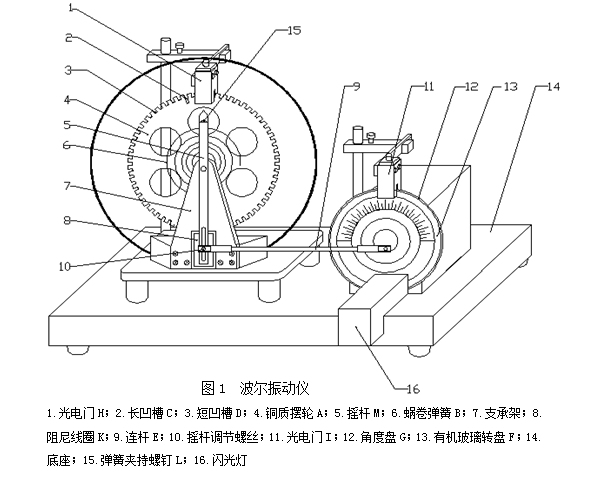
\includegraphics[scale=0.4]{device.png}
                \caption{波耳共振仪实验装置}
                % \label{fig:label}
            \end{figure}

            振动系统装有光电门通过测定缺口移动的个数来记录振动的幅度与周期,激励装置也有光电门,测定振动周期,我们可以通过调节仪器选择是否打开电机,或者改变其振动周期,并在仪器面板相应位置将其读出,
            ,还可通过调节旋钮改变阻尼大小,通过闪光灯的闪光读取有机玻璃上对应的相位角,完成实验数据的测量。
        \subsection{实验步骤}
            \subsubsection{练习1 \quad 最小阻尼时测量摆轮振动周期T与振幅$\theta$的关系}
                将阻尼开关置于最小阻尼档,打开电源开关,关掉电机和闪光灯开关,将仪器的周期选择档置于“10”位置,调节有机玻璃转盘上的0标志线指向0度,然后用手拨动摆轮使它偏离平衡位置一个大的起始角(大于120°小于180°),
                松开手后,每按一次复位键启动周期测量,就能读取10个周期的平均值,并记下这10个周期对应的首尾两次振幅值。
            \subsubsection{练习2 \quad 测量最小阻尼比}
                将周期选择档置于“1”位置,准备过程同练习1,然后用手拨动摆轮使它偏离平衡位置一个大的起始角,松手后对每k个周期读取一次振幅值$\theta_{j}=\theta_{1},\theta_{2},...,\theta_{n}$,要求$\theta_{1max}>120$,连测十个$\theta_{j}$。

                要求:
                \par{1.求出对数缩减$\Lambda$,进而求阻尼比$\xi$,直线拟合用最小二乘法。}
                \par{2.写明步骤计算不确定度$U_{\Lambda}$和$U_{\xi}$,并计算出$\tau$和Q}
                \par{3.求$\omega_{0j}=2\pi/(T_{dj}\sqrt{1-\xi^{2}})$,得$\bar{\theta_{j}}$和$\omega_{0j}$的关系}
            \subsection{练习3 \quad 测量其他阻尼档的阻尼比$\xi$等参数}
                再选5、4、3档中2到3种阻尼状态,测量振幅衰减以求$\Lambda$,要求同练习2。
            \subsection{练习4 \quad 测定受迫振动的幅频特性和相频特性曲线}
                保持练习3所置阻尼状态不变,开启电机开关,调节强迫激励周期旋钮以改变$\omega$,当振动稳定后,读出摆轮的振幅与两者之间的相位差,其中相位差通过闪光灯读取,
                在90两位差两侧分别记录8-9组数据,并将测得的相位差与振幅和理论值比较、拟合,最后做出幅频特性曲线和相频特性曲线
    % \newpage


    \section{数据处理}
        \subsection{练习1}
        \renewcommand\arraystretch{1.25}
        \begin{table}[!htbp]
            \centering
            \begin{tabular}{|c|c|c|c|c|c|c|c|} %表格8列 全部居中显示
                \hline
                \multirow{4}*{原始数据}&&1&2&3&4&5&6\\  %纵向合并4行单元格
                \cline{2-8}  %为第二列到第七列添加横线
                &$\theta_{1}$&174&161&149&146&137&121\\
                \cline{2-8}
                &$\theta_{10}$&100&110&130&118&128&94\\
                \cline{2-8}
                &10T&15.150&15.144&15.135&15.141&15.386&15.153\\
                \hline
            \end{tabular}
        \end{table}
        \begin{table}[!htbp]
            \centering
            \begin{tabular}{|c|c|c|c|c|c|c|c|} %表格8列 全部居中显示
                \hline
                \multirow{4}*{数据处理}&&1&2&3&4&5&6\\  %纵向合并4行单元格
                \cline{2-8}  %为第二列到第七列添加横线
                &$\theta_{avg}$&137&135.5&139.5&132&132.5&107.5\\
                \cline{2-8}
                &$T$&1.515&1.5144&1.5135&1.5141&1.5386&1.5153\\
                \cline{2-8}
                &$\omega$&4.147317&4.148960&4.151427&4.149782&4.083703&4.146496\\
                \hline
            \end{tabular}
        \end{table}
         初步可得固有频率$\omega_{0}=4.137948$。
        \subsection{练习2}
        \begin{table}[!htbp]
            \centering
            \begin{tabular}{|c|c|c|c|c|c|c|c|c|c|c|c|}
            \hline
            \multirow{2}{*}{原始数据} &          & 1   & 2   & 3   & 4   & 5   & 6   & 7   & 8   & 9   & 10 \\ \cline{2-12}
                                  & $\theta$ & 171 & 135 & 129 & 125 & 120 & 115 & 111 & 107 & 103 & 99 \\ \hline
            \end{tabular}
        \end{table}
        利用公式:
        $b_{1}=-K\Lambda=-K\xi\omega{0}T_{d}=\frac{-2K\pi}{\omega_{0}\sqrt{1-\xi^{2}}}\xi\omega_{0}=-2K\pi(\xi^{-2}-1)^{-0.5}$

        最小二乘法拟合ln$\theta_{i}$与i得出$b_{1}=-0.049257818$,\quad $s_{b_{1}}=0.006346937$

        其中K=5,进而求出

        $\Lambda=-\frac{b_{1}}{K}=-\frac{-0.049257818}{5}=0.0098515636$

        $\xi=[(\frac{b_{1}}{-2K\pi})^{-2}+1]^{-0.5}=[(\frac{-0.049257818}{-2*5\pi})^{-2}+1]^{-0.5}=0.00156792$

        $U_{\Lambda}=-\frac{1}{K}U_{b_{1}}\Lambda=-\frac{1}{K}t(p,v)s_{b_{1}}\Lambda=-\frac{1}{5}*2.26216*0.006346937*0.0098515636=-2.828975*10^{-5}$

        $U_{\xi}=\frac{4\pi^{2}}{4\pi^{2}+\Lambda^2}U_{\Lambda}\xi=\frac{4\pi^{2}}{4\pi^{2}+0.0098515636^{2}}*-2.828975*10^{-5}*0.00156792=-4.434499884*10^{-8}$

        $\tau=\frac{1}{\omega_{0}\xi}=\frac{1}{4.137948*0.00156792}=154.1313816$

        $Q=\frac{1}{2\xi}=\frac{1}{2*0.00156792}=318.8938211$
        \begin{figure}[ht]
            \centering
            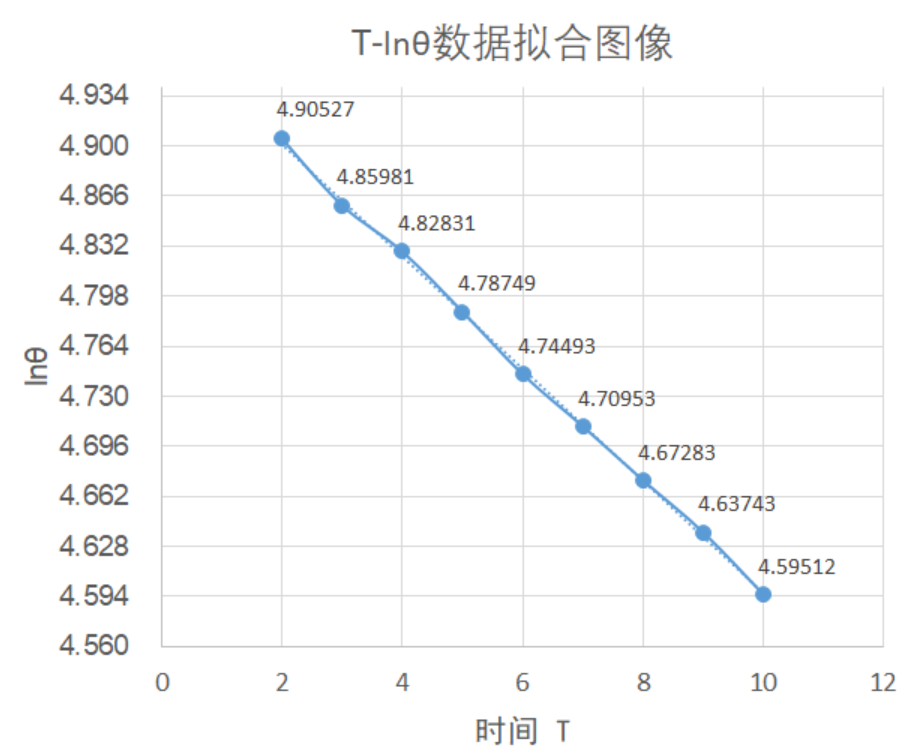
\includegraphics[scale=0.6]{second.png}
        \end{figure}
        \begin{table}[!htbp]
            \centering
            \begin{tabular}{|c|c|c|c|c|c|c|c|}
            \hline
            \multirow{4}{*}{数据处理} &               & 1        & 2        & 3        & 4        & 5         & 6        \\ \cline{2-8}
                                  & $\theta$      & 137      & 135.5    & 139.5    & 132      & 132.5     & 107.5    \\ \cline{2-8}
                                  & $\omega_{0j}$ & 4.147317 & 4.148960 & 4.151427 & 4.149782 & 4.0833703 & 4.146496 \\ \cline{2-8}
                                  & $\omega_{0}$  & 4.147322 & 4.148965 & 4.151432 & 4.149787 & 4.083708  & 4.146501 \\ \hline
            \end{tabular}
        \end{table}

        利用$\omega_{0j}=2\pi/(T_{dj}\sqrt{1-\xi^{2}})$可求出$\omega_{0j}$,对比可得$\omega_{0j}$与$\omega_{0}$几乎没有差别
        \subsection{练习3}
        \begin{table}[!htbp]
            \centering
            \begin{tabular}{|c|c|c|c|c|c|c|c|c|c|c|c|c|}
            \hline
            \multirow{4}{*}{原始数据} & 阻尼2(K=2) & 1   & 2   & 3   & 4  & 5  & 6  & 7  & 8  & 9  & 10 & 11 \\ \cline{2-13}
                                  & $\theta$ & 157 & 119 & 99  & 81 & 67 & 55 & 45 & 37 & 30 & 25 & 20 \\ \cline{2-13}
                                  & 阻尼4(K=1) & 1   & 2   & 3   & 4  & 5  & 6  & 7  & 8  & 9  & 10 & 11 \\ \cline{2-13}
                                  & $\theta$ & 149 & 119 & 101 & 86 & 73 & 62 & 53 & 45 & 37 & 32 & 27 \\ \hline
            \end{tabular}
        \end{table}
        \subsubsection{对于阻尼比为2}
        % 利用公式:
        % $b_{1_{2}}=-K\Lambda=-K\xi\omega{0}T_{d}=\frac{-2K\pi}{\omega_{0}\sqrt{1-\xi^{2}}}\xi\omega_{0}=-2K\pi(\xi^{-2}-1)^{-0.5}$

        最小二乘法拟合ln$\theta_{i}$与i得出$b_{1_{2}}=-0.200821818$,\quad $s_{b_{1_{2}}}=0.01945217$

        其中K=2,进而求出

        $\Lambda_{2}=-\frac{b_{1_{2}}}{K}=-\frac{-0.200821818}{5}=0.0401643636$

        $\xi_{2}=[(\frac{b_{1_{2}}}{-2K\pi})^{-2}+1]^{-0.5}=[(\frac{-0.200821818}{-2*2\pi})^{-2}+1]^{-0.5}=0.01597885$

        $U_{\Lambda 2}=-\frac{1}{K}U_{b_{1_{2}}}\Lambda_{2}=-\frac{1}{K}t(p,v)s_{b_{1_{2}}}\Lambda_{2}=-\frac{1}{2}*2.228138852*0.01945217*0.0401643636=-0.0008704046495$

        $U_{\xi 2}=\frac{4\pi^{2}}{4\pi^{2}+\Lambda_{2}^2}U_{\Lambda 2}\xi_{2}=\frac{4\pi^{2}}{4\pi^{2}+0.0401643636^{2}}*-0.0008704046495*0.01597885=-1.390749704*10^{-5}$

        $\tau_{2}=\frac{1}{\omega_{0}\xi_{2}}=\frac{1}{4.137948*0.01597885}=15.12409691$

        $Q_{2}=\frac{1}{2\xi_{2}}=\frac{1}{2*0.01597885}=31.29136327$
        % \newpage
        \subsubsection{对于阻尼比为4}
        % 利用公式:
        % $b_{1_{4}}=-K\Lambda=-K\xi\omega{0}T_{d}=\frac{-2K\pi}{\omega_{0}\sqrt{1-\xi^{2}}}\xi\omega_{0}=-2K\pi(\xi^{-2}-1)^{-0.5}$

        最小二乘法拟合ln$\theta_{i}$与i得出$b_{1_{4}}=-0.167474545$,\quad $s_{b_{1_{4}}}=0.001664623$

        其中K=1,进而求出

        $\Lambda_{4}=-\frac{b_{1_{4}}}{K}=-\frac{-0.167474545}{1}=0.167474545$

        $\xi_{4}=[(\frac{b_{1_{4}}}{-2K\pi})^{-2}+1]^{-0.5}=[(\frac{-0.167474545}{-2*1\pi})^{-2}+1]^{-0.5}=0.026644938$

        $U_{\Lambda 4}=-\frac{1}{K}U_{b_{1_{4}}}\Lambda_{4}=-\frac{1}{K}t(p,v)s_{b_{1_{4}}}\Lambda_{4}=-2.228138852*0.001664623*0.167474545=-6.2116496*10^{-4}$

        $U_{\xi 4}=\frac{4\pi^{2}}{4\pi^{2}+\Lambda_{4}^2}U_{\Lambda 4}\xi_{4}=\frac{4\pi^{2}}{4\pi^{2}+0.167474545^{2}}*-6.211649598*10^{-4}*0.026644938=-1.653915148*10^{-5}$

        $\tau_{4}=\frac{1}{\omega_{0}\xi_{4}}=\frac{1}{4.137948*0.026644938}=9.069853187$

        $Q_{4}=\frac{1}{2\xi_{4}}=\frac{1}{2*0.026644938}=18.76529043$

        % \newpage
        \subsection{练习4}
        \begin{table}[!htbp]
            \centering
            \begin{tabular}{|c|c|c|c|c|c|c|c|c|c|c|}
            \hline
            \multirow{8}{*}{原始数据} & 阻尼2       & 1     & 2     & 3     & 4     & 5     & 6     & 7     & 8      & 9      \\ \cline{2-11}
                                  & $\theta$  & 43    & 51    & 59    & 74    & 94    & 110   & 126   & 136    & 136    \\ \cline{2-11}
                                  & T         & 1.588 & 1.574 & 1.566 & 1.553 & 1.540 & 1.532 & 1.524 & 1.5135 & 1.5155 \\ \cline{2-11}
                                  & $\varphi$ & 18    & 23    & 25    & 33    & 43.5  & 53.5  & 66.5  & 90     & 86     \\ \cline{2-11}
                                  &           & 10    & 11    & 12    & 13    & 14    & 15    & 16    & 17     & 18     \\ \cline{2-11}
                                  & $\theta$  & 137   & 136   & 135   & 133   & 101   & 66    & 47    & 34     & 27     \\ \cline{2-11}
                                  & T         & 1.514 & 1.515 & 1.518 & 1.509 & 1.496 & 1.477 & 1.459 & 1.436  & 1.415  \\ \cline{2-11}
                                  & $\varphi$ & 89    & 87.5  & 80    & 103   & 131.5 & 149.5 & 158.5 & 163    & 165.5  \\ \hline
            \end{tabular}
            \end{table}
        \begin{table}[!htbp]
            \centering
            \begin{tabular}{|c|c|c|c|c|c|c|c|c|c|c|}
            \hline
            \multirow{8}{*}{原始数据} & 阻尼4       & 1     & 2     & 3     & 4     & 5     & 6      & 7     & 8      & 9      \\ \cline{2-11}
                                  & $\theta$  & 51    & 55    & 40    & 47    & 67    & 75     & 78    & 79     & 79     \\ \cline{2-11}
                                  & T         & 1.566 & 1.558 & 1.587 & 1.573 & 1.543 & 1.5325 & 1.523 & 1.5165 & 1.5155 \\ \cline{2-11}
                                  & $\varphi$ & 38    & 42.5  & 29    & 34    & 56    & 67     & 80    & 90     & 91     \\ \cline{2-11}
                                  &           & 10    & 11    & 12    & 13    & 14    & 15     & 16    & 17     & 18     \\ \cline{2-11}
                                  & $\theta$  & 77    & 67    & 58    & 49    & 43    & 37     & 31    & 28     & 24     \\ \cline{2-11}
                                  & T         & 1.509 & 1.492 & 1.482 & 1.471 & 1.461 & 1.449  & 1.434 & 1.424  & 1.411  \\ \cline{2-11}
                                  & $\varphi$ & 100   & 122   & 132   & 140   & 145   & 150    & 154   & 156    & 158    \\ \hline
            \end{tabular}
        \end{table}

        1)由$\omega_{0}=\frac{2\pi}{T}(\varphi=90)$可得$\omega_{0}=4.1514274$,与练习1略有差别

        2)利用$\varphi_{0}=arctan\frac{2\xi(\omega/\omega_{0})}{1-\omega^{2}/\omega_{0}^{2}}$逐点计算偏差
        \begin{table}[!htbp]
            \centering
            \begin{tabular}{|c|c|c|c|c|c|c|c|c|c|}
            \hline
            阻尼2             & 1        & 2       & 3       & 4        & 5        & 6        & 7        & 8        & 9        \\ \hline
            $\varphi$       & 18       & 23      & 25      & 33       & 43.5     & 53.5     & 66.5     & 90       & 86       \\ \hline
            $\varphi_{0}$   & 19.6244  & 23.9634 & 27.3802 & 35.3652  & 43.5625  & 55.8906  & 67.0939  & 88.2167  & 86.8928  \\ \hline
            $\Delta\varphi$ & 1.6244   & 0.9634  & 2.3802  & 2.3652   & 0.0625   & 2.3906   & 0.5939   & -1.7833  & 0.8928   \\ \hline
                            & 10       & 11      & 12      & 13       & 14       & 15       & 16       & 17       & 18       \\ \hline
            $\varphi$       & 89       & 87.5    & 80      & 103      & 131.5    & 149.5    & 158.5    & 163      & 165.5    \\ \hline
            $\varphi_{0}$   & 90.3626  & 88.0560 & 81.0159 & 101.3000 & 132.9658 & 149.9923 & 158.1933 & 164.0325 & 167.2482 \\ \hline
            $\Delta\varphi$ & 1.3626   & 0.5560  & 1.0159  & -2.3000  & 1.4658   & 0.4923   & -0.3067  & 1.0325   & 1.7482   \\ \hline
            \end{tabular}
        \end{table}
        \begin{table}[!htbp]
            \centering
            \begin{tabular}{|c|c|c|c|c|c|c|c|c|c|}
            \hline
            阻尼4             & 1        & 2        & 3        & 4        & 5        & 6        & 7        & 8         & 9        \\ \hline
            $\varphi$       & 38       & 42.5     & 29       & 34       & 56       & 67       & 80       & 90        & 91       \\ \hline
            $\varphi_{0}$   & 37.3802  & 41.8424  & 29.8827  & 34.3452  & 54.8687  & 65.0051  & 79.3491  & 90.4486   & 91.8928  \\ \hline
            $\Delta\varphi$ & -0.6198  & -0.6576  & 0.8827   & 1.3452   & -1.1313  & -1.9949  & -0.6509  & 0.4486    & 0.8928   \\ \hline
                            & 10       & 11       & 12       & 13       & 14       & 15       & 16       & 17        & 18       \\ \hline
            $\varphi$       & 100      & 122      & 132      & 140      & 145      & 150      & 154      & 156       & 158      \\ \hline
            $\varphi_{0}$   & 101.3000 & 125.6999 & 132.6583 & 143.2779 & 147.4943 & 151.1563 & 154.4028 & 156.0343  & 157.7258 \\ \hline
            $\Delta\varphi$ & 1.3000   & 0.6999   & 0.6583   & 3.2779   & 2.4943   & 1.1563   & 0.4028   & 0.0343    & -0.2742  \\ \hline
            \end{tabular}
        \end{table}
        % \newpage

        3)计算$\theta_{m}=\frac{\alpha_{m}}{\sqrt{(1-\omega^{2}/\omega_{0}^{2})^{2}+(2\xi\omega/\omega_{0})^{2}}}$并绘图
        \begin{figure}[!htbp]
            \centering
            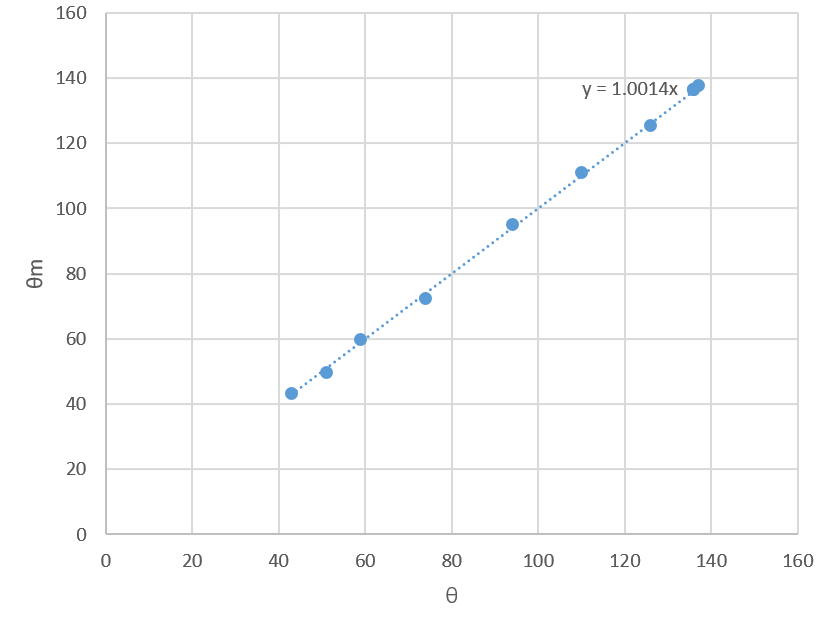
\includegraphics[scale=0.85]{fifth.png}
            \caption{阻尼2}
            % \label{fig:label}
        \end{figure}
        \begin{figure}[!htbp]
            \centering
            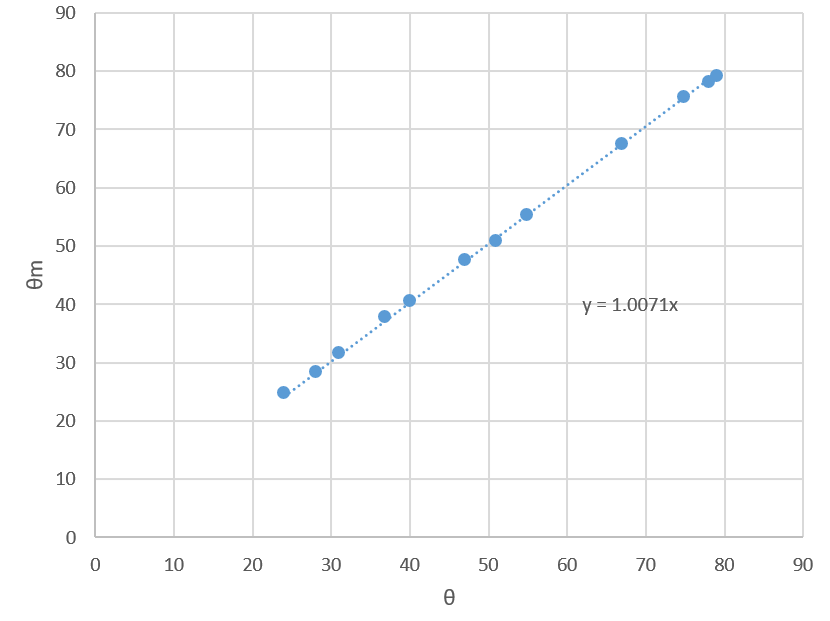
\includegraphics[scale=0.85]{fouth.png}
            \caption{阻尼4}
            % \label{fig:label}
        \end{figure}
        % \newpage

        4)绘制幅频、相频曲线
        \begin{figure}[!htbp]
            \centering
            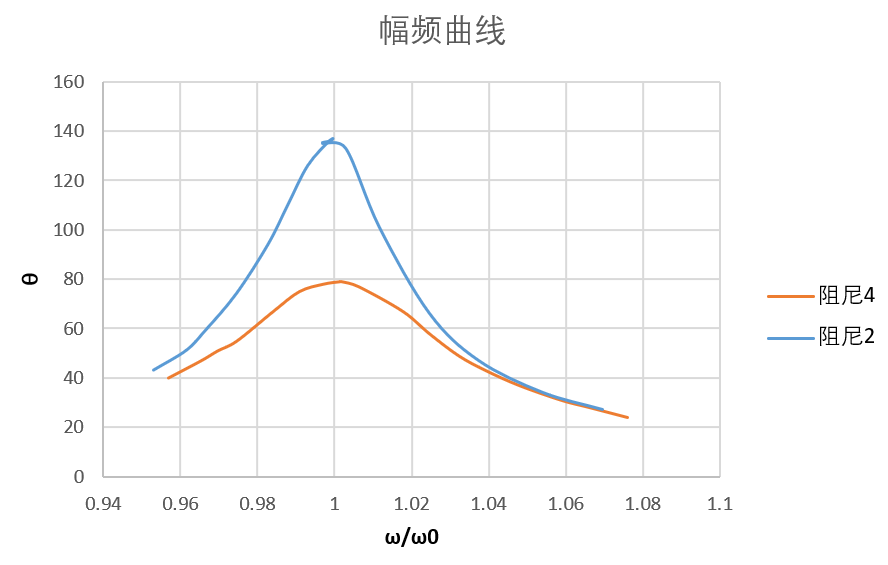
\includegraphics[scale=1.0]{sevevth.png}
            % \caption{}
            % \label{fig:label}
        \end{figure}
        \begin{figure}[!htbp]
            \centering
            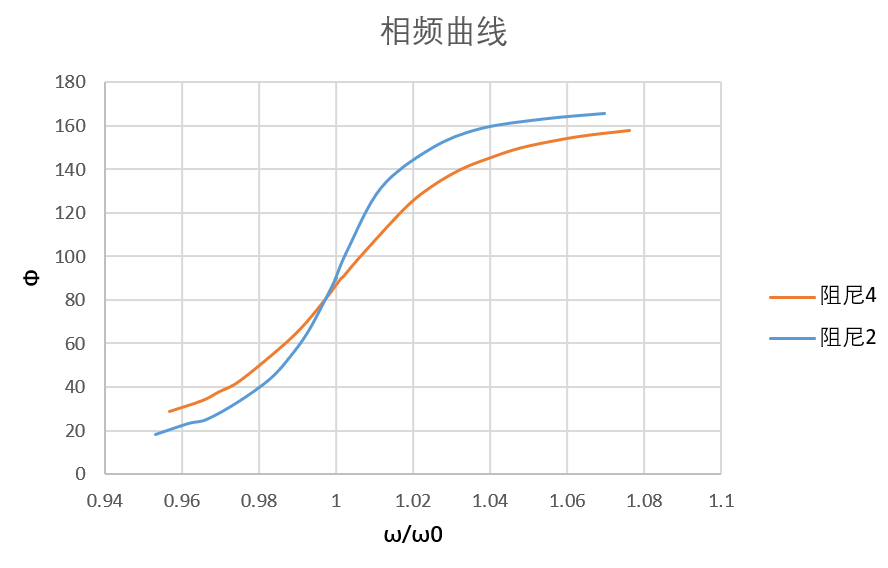
\includegraphics[scale=1.0]{sixth.png}
            % \caption{}
            % \label{fig:label}
        \end{figure}
    \section{讨论}
    本实验易于操作,但数据繁杂,处理起来很不方便,记录原始数据之前,最好事先设计表格,便于记录实验数据。处理结果与预期基本符合,但绘制曲线时发现图像对称轴并不在中心位置,
    是由于对称轴右侧数据多于左侧,要注意选点均匀,并在90附近多测几组数据。寻找90相位差时,可依据练习1的结果调节周期,方便寻找。改变阻尼时,由于剩磁会对实验影响,应连续完成练习3和4再改变阻尼状态。
    同样,闪光灯的开启也需要注意,因为有时候闪光会对振幅与周期测量产生干扰。
\end{document}
空一行为另起一段,\\为段内强制换行
